\documentclass[french, a4paper, notitlepage, 12pt]{report}

% spécifie la langue utilisée
\usepackage[english,main=french]{babel}

% permet d'entrer des caractères utf8
\usepackage[utf8]{inputenc}

% permet d'afficher correctement les caractères utf8
\usepackage[T1]{fontenc}

% permet de définir la zone de texte
\usepackage[left=3cm,right=2cm,top=2.5cm,bottom=2.5cm]{geometry}



\usepackage{helvet}
\usepackage{afterpage}
\usepackage{parskip}
\usepackage{glossaries}
\usepackage{comment}
\usepackage[page,header]{appendix}
\usepackage{titletoc}
\usepackage{lipsum}
\usepackage{caption}
\usepackage{eurosym}
\usepackage{array,multirow,makecell}
\usepackage{booktabs}



% permet d'ajouter des images présent dans le fichier
\usepackage{graphicx}
\graphicspath{ {./rsc/} }

% permettre de cliquer sur les tables de matière et les références
\usepackage{hyperref}

% permet d'indenter le paragraphe
\usepackage[raggedright]{titlesec}
\titleformat{\paragraph}[hang]{\normalfont\normalsize\bfseries}{\theparagraph}{1em}{}
\titlespacing*{\paragraph}{0pt}{3.25ex plus 1ex minus .2ex}{0.5em}

% permet d'écrire du code avec un cadre
\usepackage{listings}
\lstset{
numbers=left,
numberstyle=\small,
numbersep=8pt,
frame = single,
language=Pascal,
framexleftmargin=15pt,
basicstyle=\small,
literate={á}{{\'a}}1 {ã}{{\~a}}1 {é}{{\'e}}1,
}

 % indenter les paragraphe
\usepackage{indentfirst}
\setlength{\parindent}{0.5cm}

% numérotation qui se suit dans la table des figures et table des tableaux
\usepackage{chngcntr}
\counterwithout{figure}{chapter}
\counterwithout{table}{chapter}

% permet d'enlever les espaces dans la table des figures et la table des tableaux entre chaque chapitre
\makeatletter
\def\@chapter[#1]#2{\ifnum \c@secnumdepth >\m@ne
                       \if@mainmatter
                         \refstepcounter{chapter}%
                         \typeout{\@chapapp\space\thechapter.}%
                         \addcontentsline{toc}{chapter}%
                                   {\protect\numberline{\thechapter}#1}%
                       \else
                         \addcontentsline{toc}{chapter}{#1}%
                       \fi
                    \else
                      \addcontentsline{toc}{chapter}{#1}%
                    \fi
                    \chaptermark{#1}%
                    \if@twocolumn
                      \@topnewpage[\@makechapterhead{#2}]%
                    \else
                      \@makechapterhead{#2}%
                      \@afterheading
                    \fi}
\makeatother

% renomme table en tableau
\addto\captionsfrench{\def\tablename{Tableau}}

% permet d'ajouter des tableaux
\usepackage{array,multirow,makecell}
\setcellgapes{1pt}
\makegapedcells
\newcolumntype{R}[1]{>{\raggedleft\arraybackslash }b{#1}}
\newcolumntype{L}[1]{>{\raggedright\arraybackslash }b{#1}}
\newcolumntype{C}[1]{>{\centering\arraybackslash }b{#1}}
\newcommand\tabitem{~~\llap{\textbullet}~~}

\newacronym{GHT}{GHT}{Groupement Hospitalier de Territoire}
\newacronym[plural=ESPIC,firstplural=Établissements de Santé Privé d’Intérêt Collectif (ESPIC)]{ESPIC}{ESPIC}{Établissement de Santé Privé d’Intérêt Collectif}

\newcommand\emptyPage {
    \null
    \thispagestyle{empty}
    \addtocounter{page}{-1}
    \newpage
}

\renewcommand\contentsname{Table des matières}\setcounter{secnumdepth}{5}
\renewcommand\listfigurename{Table des figures}
\renewcommand\listtablename{Table des tableaux}

\renewcommand\thefigure{\arabic{figure}}
\setcounter{figure}{0}

\renewcommand\thetable{\arabic{table}}
\setcounter{table}{0}

\makeglossaries
\begin{document}
\begin{titlepage}
  \thispagestyle{empty}

  \begin{minipage}{0.45\textwidth}
    \begin{flushleft}
      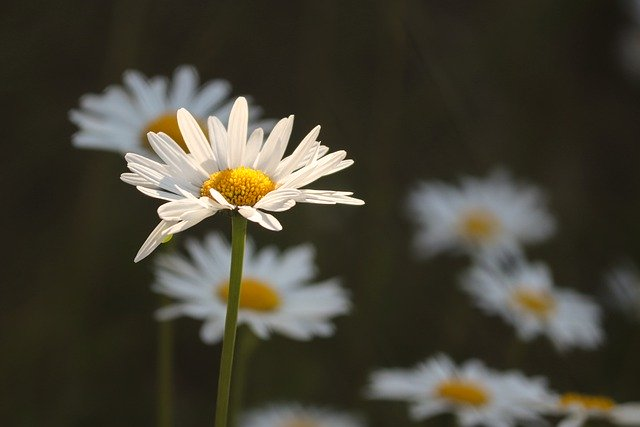
\includegraphics[width=5cm]{img.jpg}
    \end{flushleft}
  \end{minipage}
  \begin{minipage}{0.45\textwidth}
    \begin{flushright}
      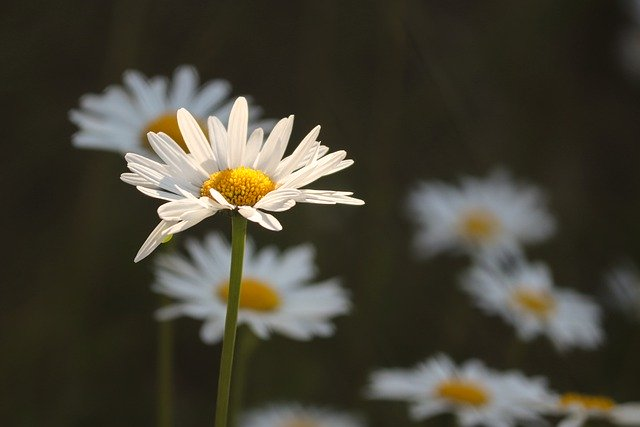
\includegraphics[width=4cm]{img.jpg}
    \end{flushright}
  \end{minipage}\\[3cm]

  \newcommand{\HRule}{\rule{\linewidth}{0.5mm}}
  \center

  \textsc{\Large Diplôme}\\
  \textsc{\Large Spécialité}\\
  \textsc{\large .... - ....}\\[2cm]
  \textsc{\Large Rapport de stage du ../../.... au ../../....}\\[.5cm]

  \HRule \\[0.4cm]
  { \huge \bfseries Titre stage}\\[0.1cm]
  \textsc{\large sous titre}\\
  \HRule \\[3cm]

  \begin{minipage}{0.4\textwidth}
    \begin{flushleft} \large
      \emph{Réalisé par:}\\
      \textsc{...}
    \end{flushleft}
  \end{minipage}
  \begin{minipage}{0.4\textwidth}
    \begin{flushright} \large
      \emph{Tuteur en entreprise:} \\
      \textsc{...} \\ [1cm]
      \emph{Tuteur universitaire:} \\
      \textsc{...} \\
    \end{flushright}
  \end{minipage}
  \vfill
  \clearpage
\end{titlepage}

\emptyPage

\chapter*{Remerciements}\addcontentsline{toc}{chapter}{Remerciements}

\startcontents
\printcontents{}{0}{\chapter*{\hspace*{1.2em}\contentsname}}

\addcontentsline{toc}{chapter}{Table des figures}
\listoffigures

\addcontentsline{toc}{chapter}{Table des tableaux}
\listoftables

\addcontentsline{toc}{chapter}{Glossaire}
\printglossaries

\chapter*{Introduction}\addcontentsline{toc}{chapter}{Introduction}

\chapter{Entreprise}

\section{Présentation}

\begin{figure}[h]
  \begin{center}
    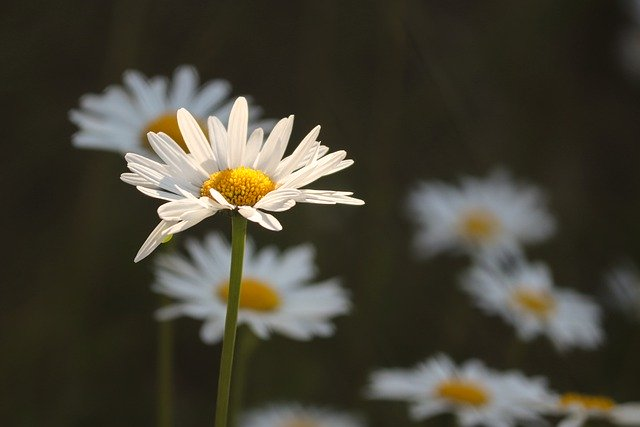
\includegraphics[scale=0.44]{img.jpg}
    \captionof{figure}{c'est une image}
    \label{fig1}
  \end{center}
\end{figure}

nanana

figure \ref{fig1}

tableau \ref{prio}

\textit{text anglais}.

\og guillemet\fg{}

\gls{GHT}

\glspl{ESPIC}

\cite{ref1}.

\section{section1}

\begin{itemize}
  \item item1 ;
  \item item2.
\end{itemize}

\begin{description}
  \item [1 :] nananaa.
  \item [2 :] nananaa.
\end{description}

\section{section2}

\begin{table}[h]
  \selectlanguage{french}
  \begin{center}
    \begin{tabular}{C{2.2cm}|C{2.2cm} C{2.2cm} C{2.2cm} C{2.2cm} C{2.2cm}}
                  & Inévitable & Fréquent & Occasionnel & Rare & Non~définie \\ \hline
      Bloquant    & 1          & 1        & 2           & 3    & 4           \\
      Majeur      & 1          & 2        & 2           & 4    & 4           \\
      Mineur      & 2          & 2        & 3           & 4    & 4           \\
      Cosmétique  & 3          & 4        & 4           & 4    & 4           \\
      Non~définie & 4          & 4        & 4           & 4    & 4           \\
    \end{tabular}
    \captionof{table}{Définition des priorités}
    \label{prio}
  \end{center}
\end{table}

\newpage

\begin{figure}[h]
  \begin{lstlisting}
{
    code
}
  \end{lstlisting}
  \caption{c'est du code}
  \label{code1}
\end{figure}

\chapter{Bilan}

\chapter*{Conclusion}\addcontentsline{toc}{chapter}{Conclusion}


\renewcommand\bibname{Netographie}\addcontentsline{toc}{chapter}{Netographie}
\bibliographystyle{unsrt}
\bibliography{netographie}

% annexes
\appendix\addcontentsline{toc}{chapter}{Table des annexes}
\startcontents
\renewcommand\contentsname{Table des annexes}
\printcontents{}{0}{\chapter*{\hspace*{1.2em}\contentsname}}
\setcounter{chapter}{0}

\chapter*{Annexe 1}\addcontentsline{toc}{chapter}{Annexe 1}
\pagenumbering{Roman}
\setcounter{page}{1}

\newpage
\thispagestyle{empty}
\vspace*{\stretch{1}}
\begin{otherlanguage}{french}
  \begin{abstract}
    resumé fr
  \end{abstract}

  MotClé1 – MotClé2
\end{otherlanguage}

\begin{otherlanguage}{english}
  \begin{abstract}
    resumé en
  \end{abstract}
  MotClé1 – MotClé2
\end{otherlanguage}
\vspace*{\stretch{1}}

\end{document}
